\documentclass{article}

\usepackage{graphicx}
\usepackage{amsmath}
\usepackage{siunitx}
\usepackage{xcolor}
\usepackage{tikz}
\usepackage[english,german]{babel}

\definecolor{yucky}{HTML}{dee2e6}
\definecolor{yuckytext}{HTML}{343a40}

\usetikzlibrary{shapes,arrows}

\tikzstyle{decision} = [diamond, draw, fill=blue!20,
    text width=4.5em, text badly centered, node distance=3cm, inner sep=0pt]
\tikzstyle{block} = [rectangle, draw=yucky, fill=yucky, text=yuckytext,
    text width=10em, text centered, rounded corners, minimum height=4em, minimum width=10em]
\tikzstyle{line} = [draw, -latex']
\tikzstyle{cloud} = [draw, ellipse,fill=red!20, node distance=3cm,
    minimum height=2em]

\newcommand\equalhat{\mathrel{\stackon[1.5pt]{=}{\stretchto{%
    \scalerel*[\widthof{=}]{\wedge}{\rule{1ex}{3ex}}}{0.5ex}}}}

\begin{document}

\begin{center}
\Large{Messtechnikversuch: Blutdruckmessung}
\end{center}

\begin{flushright}
  R. Grünert\\
  02.10.2020
\end{flushright}

\section{Messaufbau / -ablauf}
\begin{center}
\begin{tikzpicture}[node distance = 2cm, auto]
    % Place nodes
    \node [block] (init) {Blutdruck-\\messgerät / Kompressor};
    \node [block, below of=init] (identify) {T-Stück, Drucksensor \\ $6.4\,\frac{\si{\milli\volt}}{100 \, \si{mm} \text{Hg}}$};
    \node [block, below of=identify] (evaluate) {Widerstands-\\messbrücke};
    \node [block, below of=evaluate] (decide) {Instrumenten-\\verstärker\\ $V = 67.77$};
    \node [block, below of=decide, node distance=3cm] (stop) {CSV, Offsetkorrektur, digitale Filterung, Messwertbestimmung, etc.};
    % Draw edges
    \path [line] (init) -- (identify);
    \path [line] (identify) -- (evaluate);
    \path [line] (evaluate) -- (decide);
    \path [line] (decide) -- (stop);
\end{tikzpicture}
\end{center}

Ziel: Ermittlung des systolischen und diastolischen Blutdruckes sowie der Herzfrequenz durch Druckmessung.\\

\subsection{Messung}
Bei der Messung sollte darauf geachtet werden, dass man möglichst ruhig sitzt, da leichte Muskelkontraktionen bereits zu Abweichungen führen. Dies ist z.B. am Ende der vorliegenden Messung erkennbar, da dort die Manschette frühzeitig abgenommen wurde.

\subsubsection{Daten des Blutdruckmessgerätes}
Vom Messgerät ermittelte Werte:\\
Systolisch: 153\\
Diastolisch: 87\\
Herzrate: 73 bpm

\subsubsection{Oszilloskopdaten}

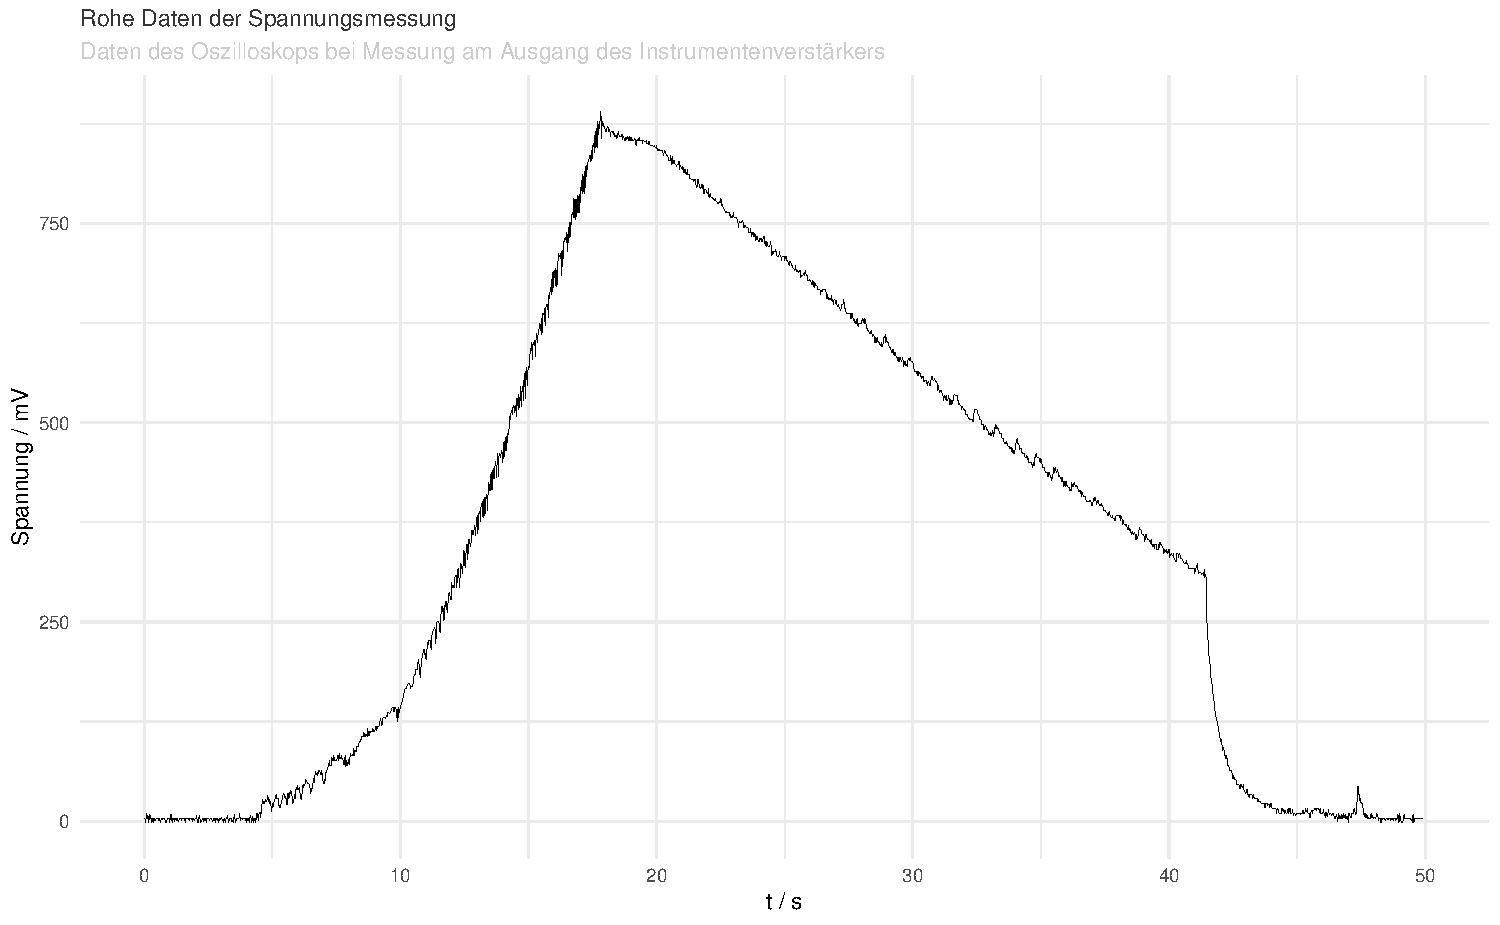
\includegraphics[width=\textwidth]{graphics/raw_data.pdf}

\noindent{Einstellungen:}
hor: $5 \, \dfrac{\si{\second}}{\text{div}}$, vert: $150 \, \frac{\si{\milli\volt}}{\si{div}}$

\noindent{{Abtastfrequenz:}}

\[ T_{\text{sample}} = \frac{5 \, \dfrac{\si{\second}}{\text{div}} \cdot 10 \, \text{div}}{2000 \, \text{samples}} = 25 \, \si{\milli\second}\]

\[\rightarrow f_{\text{sample}} = 40 \, \si{\hertz}\]

\section{Nachbereitung der Daten}

\subsection{Offsetkorrektur}
Ermittlung des vertikalen Offsets $O$ durch Mittelung der Messwerte am Ende der Messung, inetwa ab $t = 48 \, \si{\second}$ (Entspricht dem 1916. Messwert). Danach Abzug dieses Offsets (system. Fehler) von den einzelnen Messwerten.

\[O = \frac{1}{2000 - 1916} \sum^{2000}_{i=1916}{x_{i}} = 3.3 \, \si{\milli\volt}\]

\subsection{Filterung}
FIR-Tiefpass-Filterung mit Grenzfrequenz bei $f_{g} = 4 \, \si{\hertz}$, dies entspricht $240 \, \si{bpm}$.

\subsection{Regression}

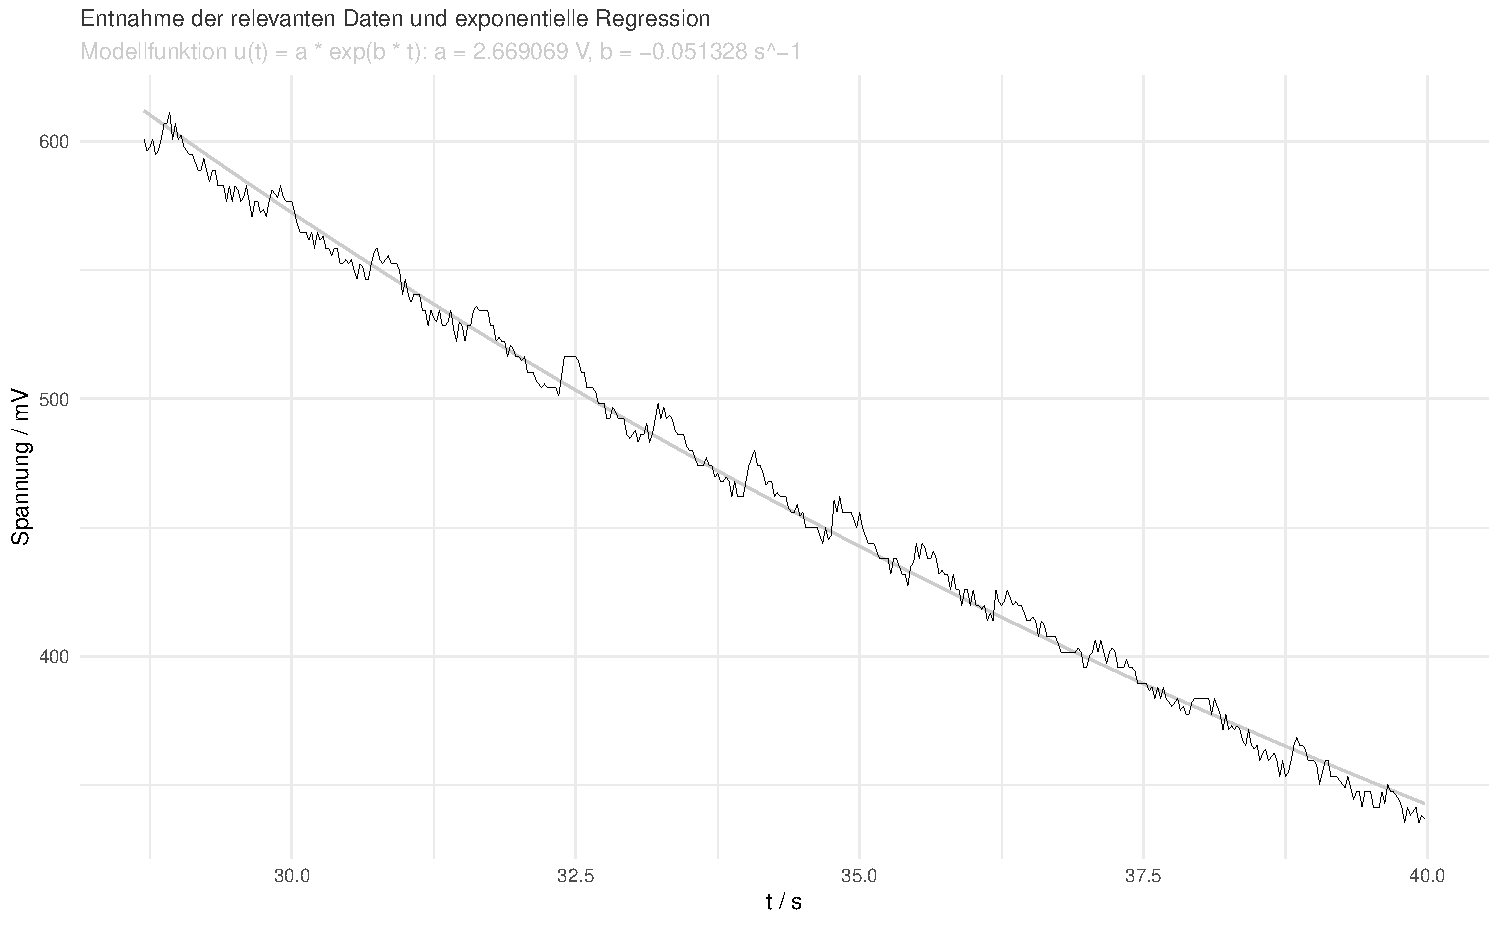
\includegraphics[width=\textwidth]{graphics/regression.pdf}

Der relevante Bereich der Messung wurde über die Größe der \glqq Amplituden \grqq ermittelt und befindet sich für die vorliegenden Messwerte zwischen dem 1149. und dem 1600. Messwert. Dieser folgt einer exponentiell abklingenden Funktion. Durch Ermittlung der Regressionsfunktion nach der Methode der kleinsten Fehlerquadrate kann diese Funktion von den Messwerten abgezogen werden, um einen klaren Verlauf des Druckunterschiedes (bzw. der Spannung) zu erhalten.\\

In diesem Fall ist die Regressionsfunktion
\[r(t) = 2.669 \si{\volt} \cdot e^{-0.0513 \si{\second}^{-1} \cdot t}\]

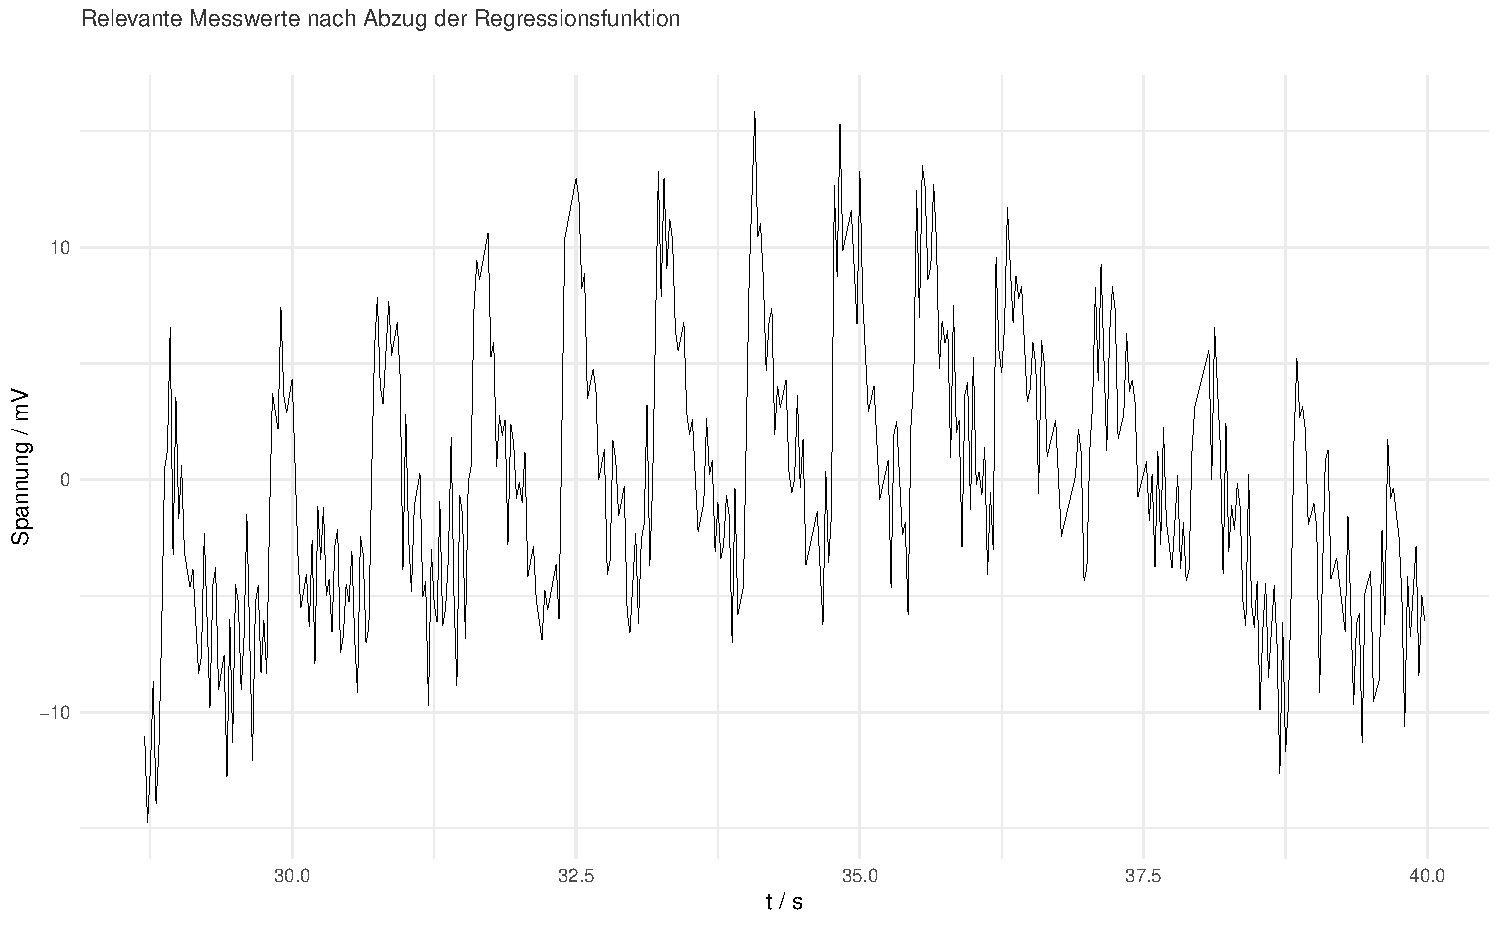
\includegraphics[width=\textwidth]{graphics/extraction.pdf}

\subsection{Herzfrequenz}

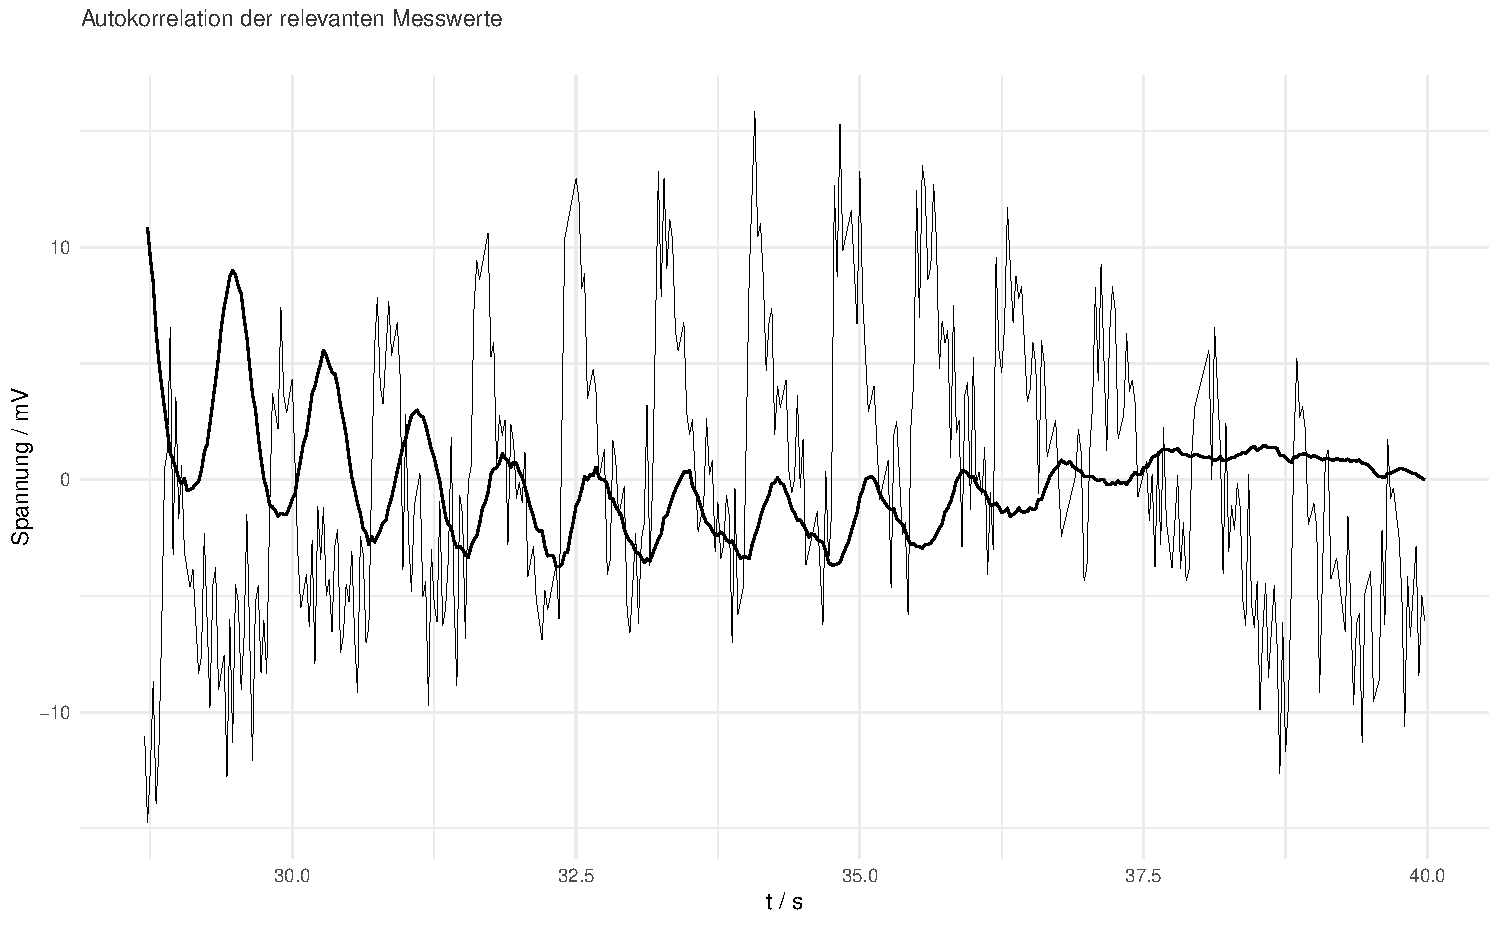
\includegraphics[width=\textwidth]{graphics/correlation.pdf}

Die Autokorrelation dieses Verlaufes weist ebenfalls einen periodischen Verlauf auf. Es gibt nun zwei Vorgehensweisen, um die Herzfrequenz zu bestimmen.

\subsubsection{Periodendauer}
Im Zeitbereich kann man die Auftretenszeiten zweier aufeinanderfolgender Spitzen der Autokorrelation bestimmen, aus der Differenz die Periodendauer und aus deren Kehrwert die Herzfrequenz bestimmen.

\[\Delta t = 33.483 - 32.689 = 0.794\]
\[f_{\text{ZB}} = \frac{1}{\Delta t} = 1.2595 \, \si{\hertz} = 75.57 \, \si{bpm}\]

\subsubsection{FFT}
Mithilfe der DFT der Autokorrelationsfunktion kann man die Herzfrequenz ebenfalls bestimmen.

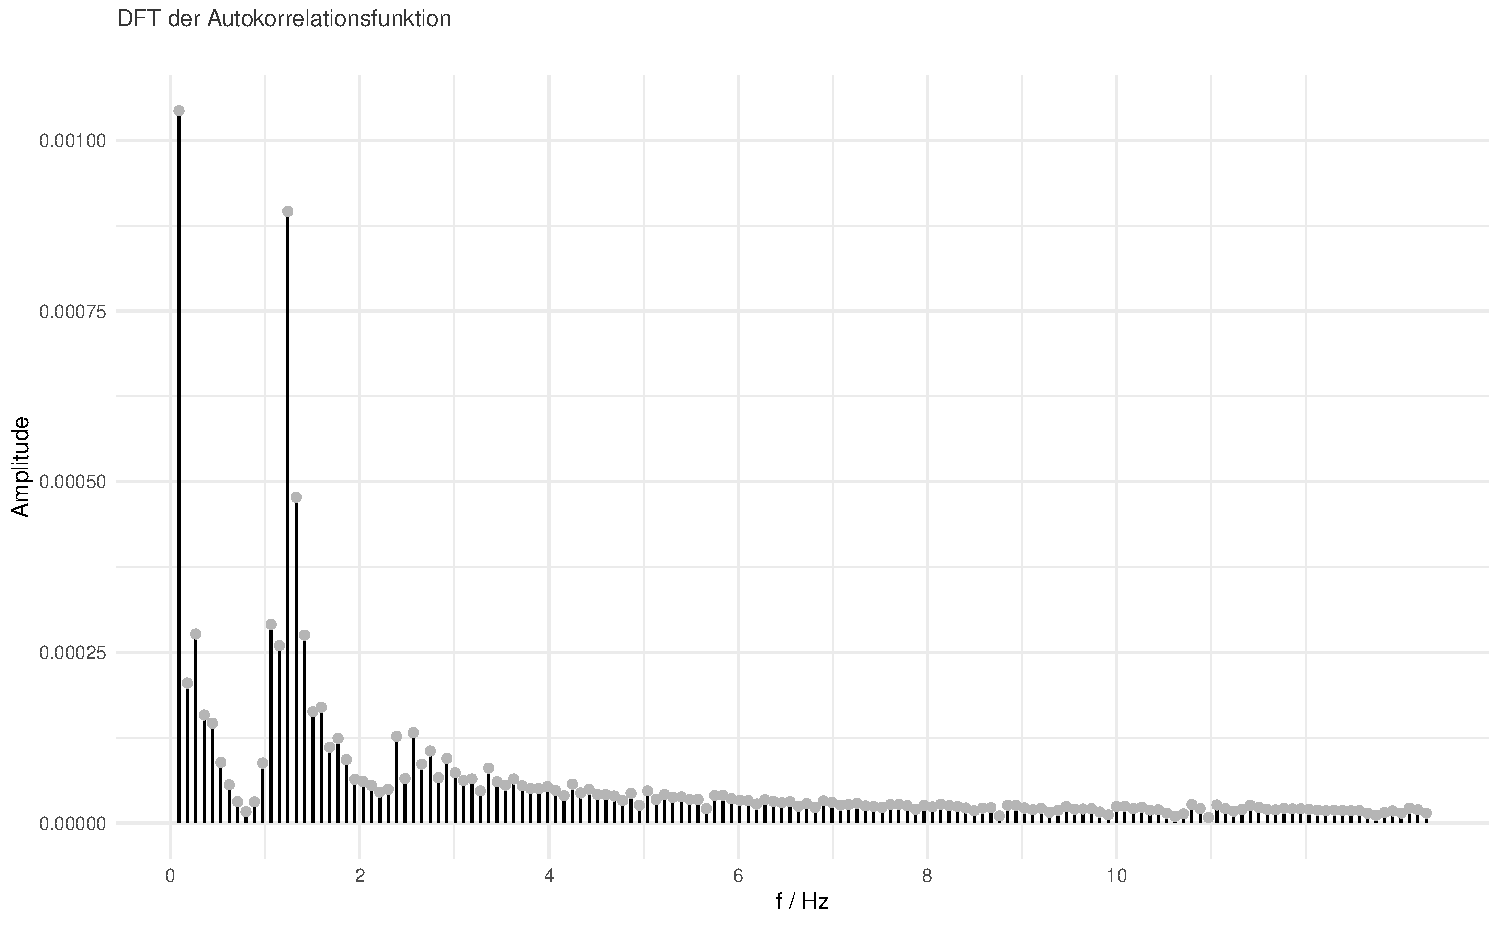
\includegraphics[width=\textwidth]{graphics/corr_fft.pdf}

\end{document}
